\documentclass[]{article}

% Imported Packages
%------------------------------------------------------------------------------
\usepackage{amssymb}
\usepackage{amstext}
\usepackage{amsthm}
\usepackage{amsmath}
\usepackage{enumerate}
% \usepackage{enumitem}
\usepackage{fancyhdr}
\usepackage[margin=1in]{geometry}
\usepackage{graphicx}
%\usepackage{extarrows}
%\usepackage{setspace}
%\usepackage{xcolor}
\usepackage{color}
\usepackage{longtable}
\usepackage{booktabs}
\usepackage{float}
% \usepackage{biblatex}
% \usepackage[backend=biber,style=ieee]{biblatex} % Ensure 'style=ieee' is set
% \addbibresource{references.bib} % Add your bibliography file
\numberwithin{figure}{section} % Enables section-based figure numbering

%------------------------------------------------------------------------------

% Header and Footer
%------------------------------------------------------------------------------
\pagestyle{plain}  
\renewcommand\headrulewidth{0.4pt}                                      
\renewcommand\footrulewidth{0.4pt}                                    
%------------------------------------------------------------------------------

% Title Details
%------------------------------------------------------------------------------
\title{Deliverable \#1: Software Requirement Specification (\textbf{SRS})}
\author{SE 3A04: Software Design II -- Large System Design}
\date{}
                            
%------------------------------------------------------------------------------

% Document
%------------------------------------------------------------------------------
\begin{document}

\maketitle	
\noindent{\bf Tutorial Number:} T02\\
{\bf Group Number:} Group 5 \\
{\bf Group Members:} 
\begin{itemize}
	\item Sarah Dorfman
	\item Gurmanjot Minhas
	\item Cheukman Zhou
	\item Ke Ma
	\item Andy Huynh (Leader)
\end{itemize}

% SECTION 1 
\section{Introduction}
\label{sec:introduction}
% Begin Section


\subsection{Purpose}
\label{sub:purpose}
% Begin SubSection
The purpose of the \textbf{SRS} is to serve as an outline of \textbf{Languify} for the developers, clients, and other stakeholders. It provides these stakeholders with a broad understanding of the requirements and design considerations. Section 1 establishes the scope of the product and defines any terms or references that will be mentioned in the rest of the document.
% End SubSection


\subsection{Scope}
\label{sub:scope}
% Begin SubSection
The product is a mobile app called \textbf{Languify} that takes an input from the user and identifies the language. 
A User Interface takes in a written text input in the form of a PDF document, image, or typed text. 
The input is then sent to a backend server called the Expert Manager that communicates with 3 different \textbf{experts} who specify what language they believe the input is. 
The User Interface will interact with the Controller, which interacts with two components.
These components are the data structure Language Info, which stores facts about different languages, and Layout Rules, which acts as a knowledge source on how to lay out the data.\\ \\
The \textbf{experts} are skilled at specific scripts or categories of script and identifying languages from those groups. The first expert identifies languages that use the Latin script, such as English and German. 
The second expert specifies in languages that use the Arabic script, such as Arabic and Urdu \cite{Britannica2025_WritingSystems}. The third expert specializes in languages that have a unique script, such as Korean which is the only widely spoken language that uses Hangul \cite{Britannica2025_Hangul}. \\ \\
The product only identifies languages that use Latin, Arabic, and unique scripts. It will only identify the 100 most spoken languages \cite{Ethnologue2025}. It does not distinguish between different dialects. As an innovative feature, the app displays some general information about the identified language, such as the number of speakers and some common phrases.\\ \\
The application is useful for people who are frequently exposed to languages they do not know. This is primarily for people who live in diverse regions or travellers. It is great for those who are curious about other cultures and may want to know some basic information to use. It encourages this curiosity and allows users to connect across cultural barriers. The overall goal is to make this product as accessible as possible.
% End SubSection


\subsection{Definitions, Acronyms, and Abbreviations}
\label{sub:definitions_acronyms_and_abbreviations}
% Begin SubSection
\begin{itemize}
	\item \textbf{AODA} – Accessibility for Ontarians with Disabilities Act
	\item \textbf{API} – Application Programming Interface
	\item \textbf{ISO} – International Organization for Standardization
	\item \textbf{Languify} – The name of the application that users shall recognize.
	\item \textbf{MVP} – The minimal viable product, which is a basic and usable version of the product. 
	\item \textbf{PIPEDA} – Personal Information Protection and Electronic Documents Act
	\item \textbf{SRS} – The software requirements specification, which is this document.
	\item \textbf{Agents/Experts} – Knowledge sources that help validate the correct language
\end{itemize}
% End SubSection


\subsection{References}
\label{sub:references}
% Begin SubSection
% \begin{itemize}
\printbibliography
% \bibliographystyle{IEEEtran}
% \bibliography{references}
% End SubSection


\subsection{Overview}
\label{sub:overview}
% Begin SubSection
The remainder of this document delves further into further details about the requirements specification. Section 2 is the overall product description and provides users with a general understanding of this product. This section discusses the product perspective, product functions, user characteristics, constraints, assumptions and dependencies, and apportioning of requirements. Section 3 provides a use case diagram that demonstrates how users will interact with the application. Section 4 supplements Section 3 by going into detail about functional requirements. This section also details all the main business events and viewpoints. Finally, Section 5 lists non-functional requirements and justifies their inclusion.
% End SubSection

% End Section


% SECTION 2
\section{State Charts For Controller Classes}
\label{sec:stateChartsForControllerClasses}

\begin{figure}[H]
	\centering
	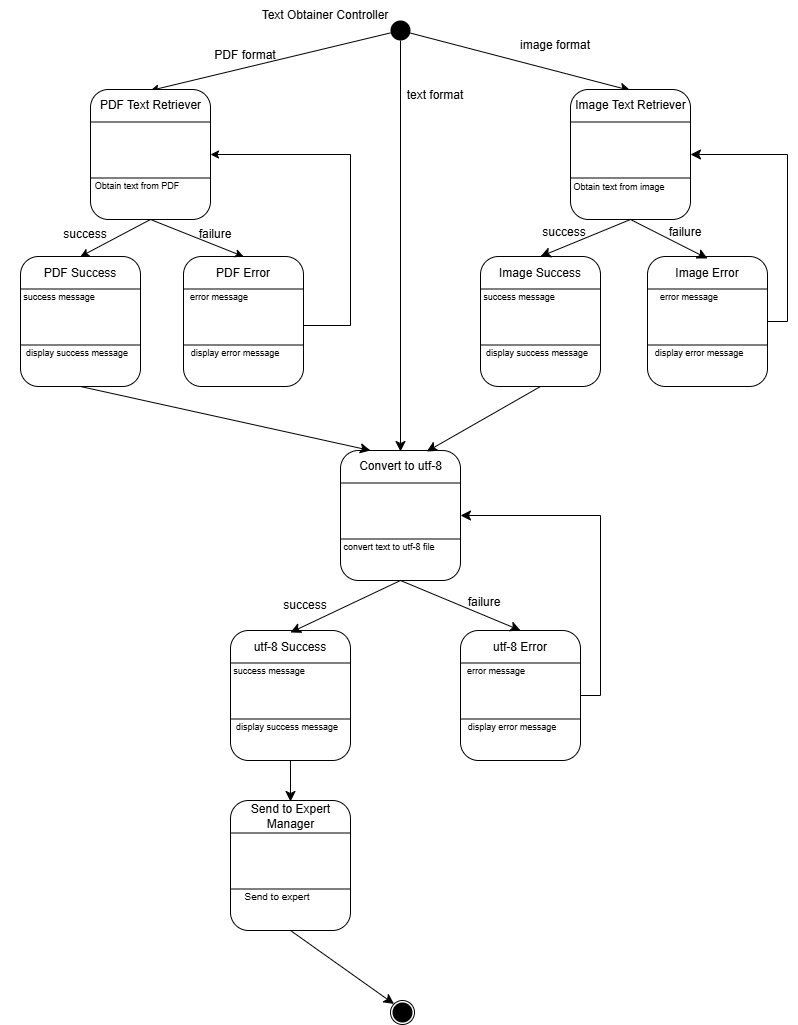
\includegraphics[width=\textwidth, height=\textheight]{Section2/images/text_obtainer_state_diagram.png}
	\caption{Text Obtainer}
	\label{TextObtainer}
\end{figure}
\begin{figure}[H]
	\centering
	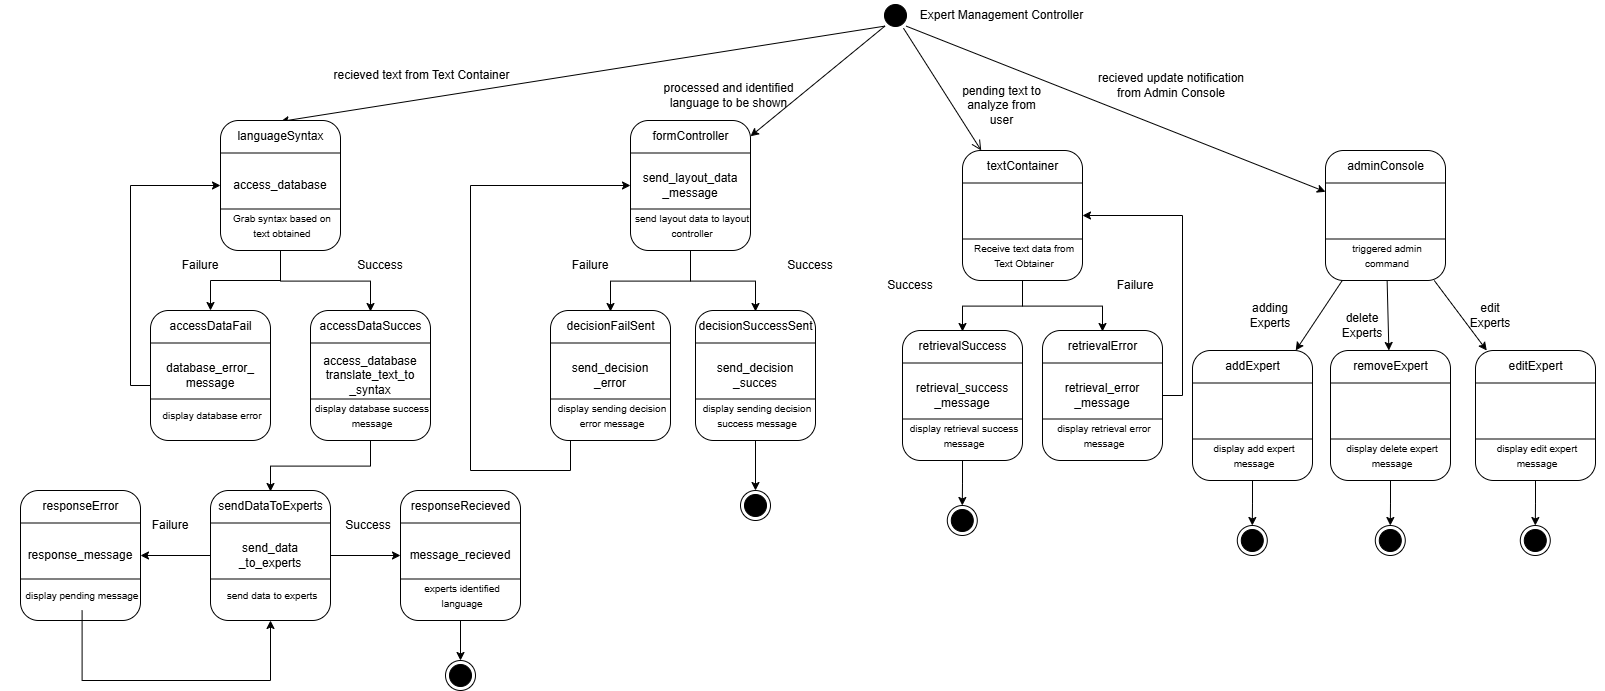
\includegraphics[width=\textwidth, height=\textheight, keepaspectratio]{Section2/images/Expert_Manager_state_diagramV3.png}
	% 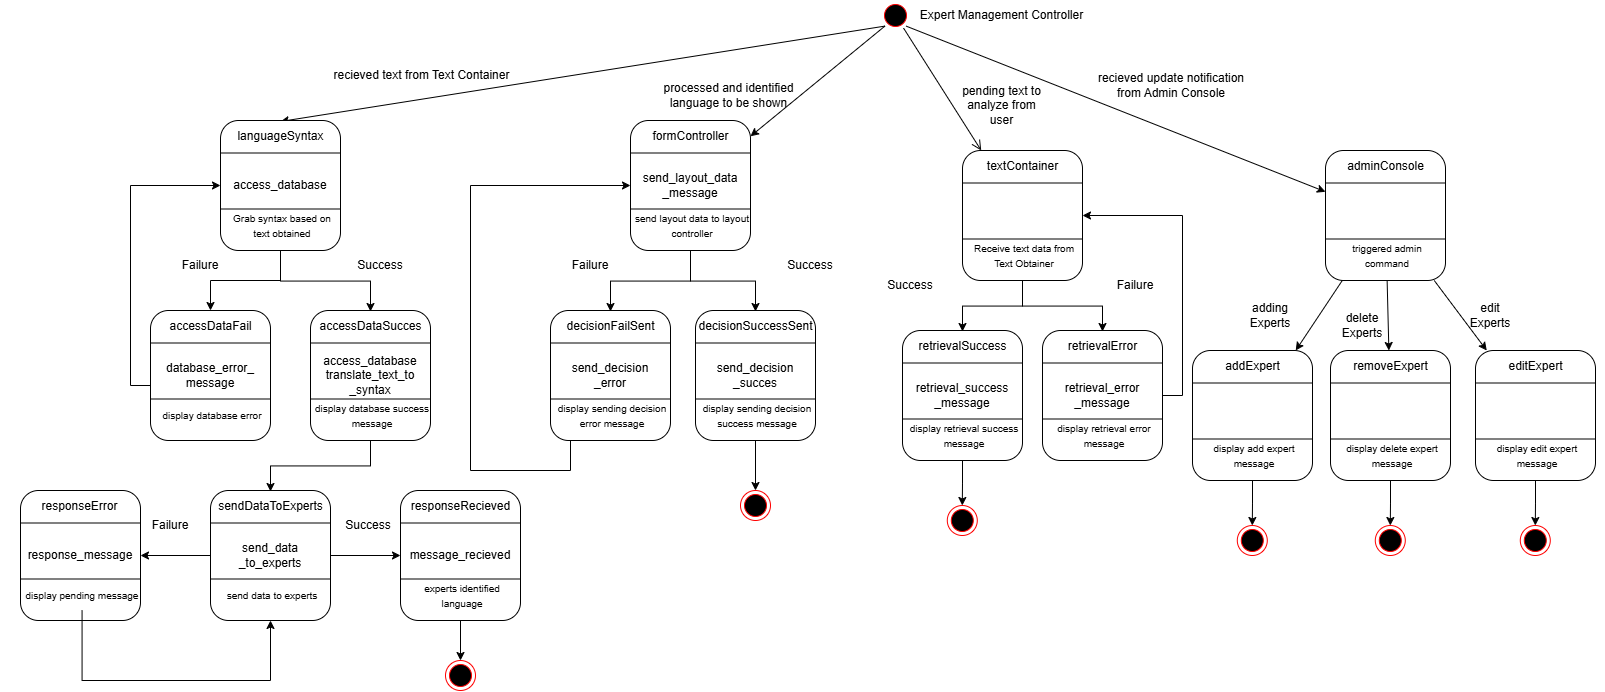
\includegraphics[width=\linewidth, trim=0.5\width 0.1\height 0 0, clip]{Section2/Expert_Manager_state_diagram.png}
	\caption{Expert Manager}
	\label{ExpertManager}
\end{figure}

\begin{figure}[H]
	\centering
	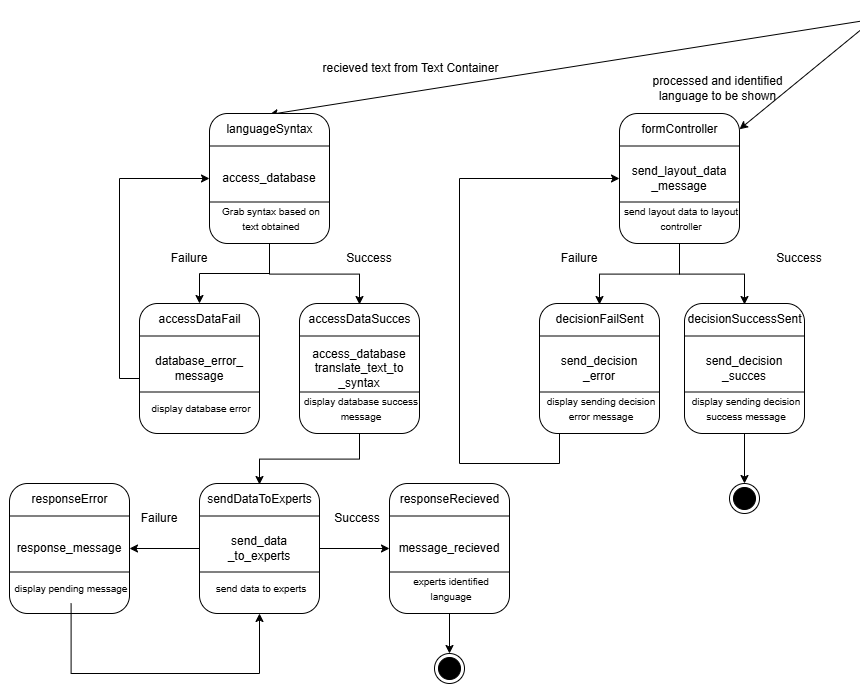
\includegraphics[width=\textwidth, height=\textheight, keepaspectratio]{Section2/images/Expert_Manager_state_diagramV3_left_half.png}
	% 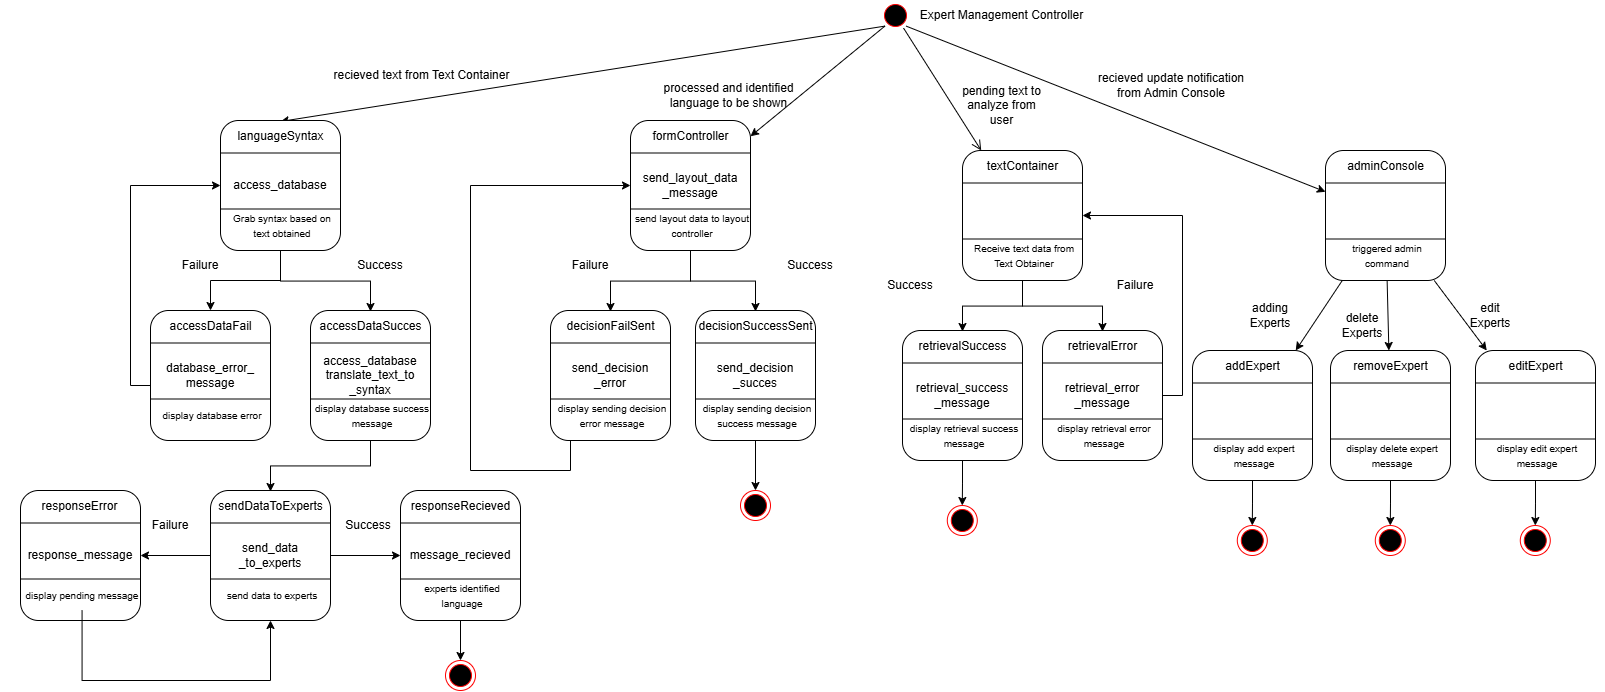
\includegraphics[width=\linewidth, trim=0.5\width 0.1\height 0 0, clip]{Section2/Expert_Manager_state_diagram.png}
	\caption{Expert Manager Left Half}
	\label{ExpertManagerp1}
\end{figure}


\begin{figure}[H]
	\centering
	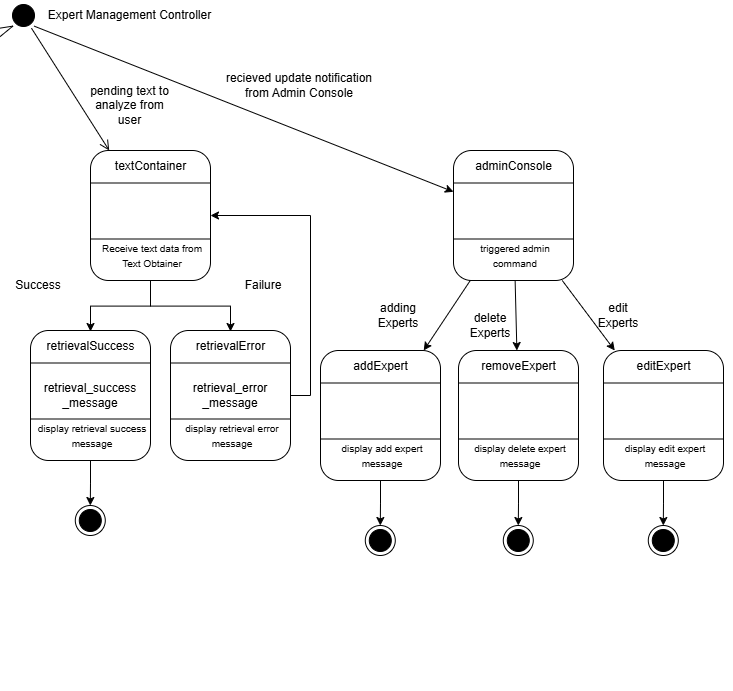
\includegraphics[width=\textwidth, height=\textheight, keepaspectratio]{Section2/images/Expert_Manager_state_diagramV3_right_half.png}
	% 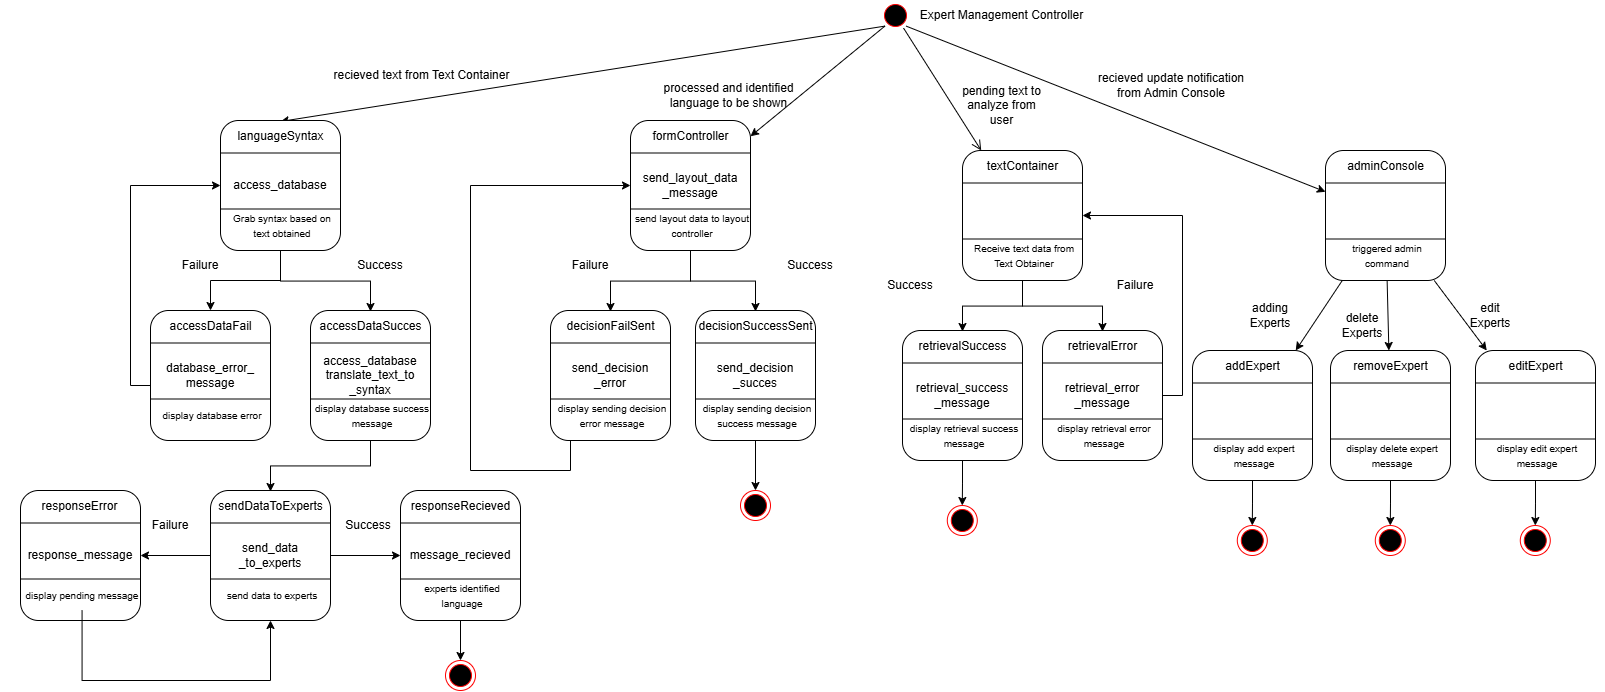
\includegraphics[width=\linewidth, trim=0.5\width 0.1\height 0 0, clip]{Section2/Expert_Manager_state_diagram.png}
	\caption{Expert Manager Right Half}
	\label{ExpertManagerp1}
\end{figure}
\begin{figure}[H]
	\centering
	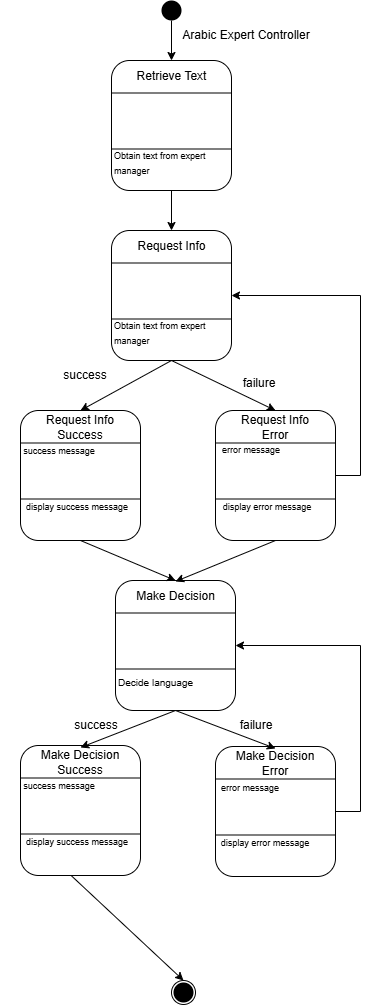
\includegraphics[width=\textwidth, height=0.95\textheight, keepaspectratio]{Section2/images/arabic_expert_state_diagram.png}
	\caption{Arabic Expert}
	\label{ArabicExpert}
\end{figure}
\begin{figure}[H]
	\centering
	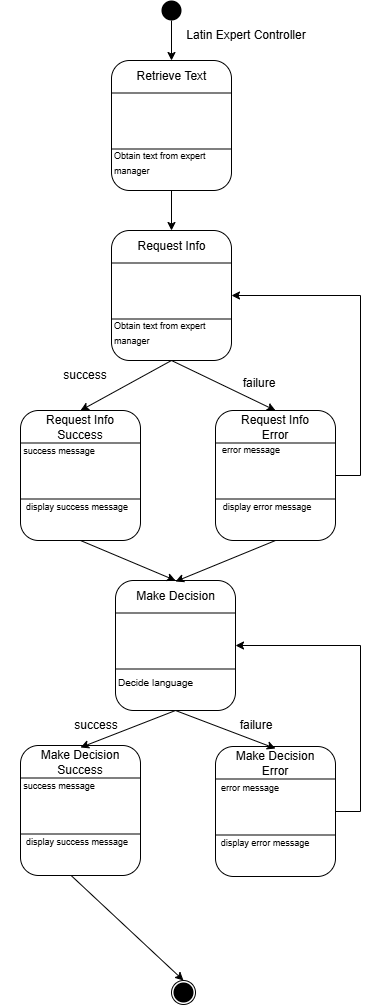
\includegraphics[width=\textwidth, height=\textheight, keepaspectratio]{Section2/images/latin_expert_state_diagram.png}
	\caption{Latin Expert}
	\label{LatinExpert}
\end{figure}
\begin{figure}[H]
	\centering
	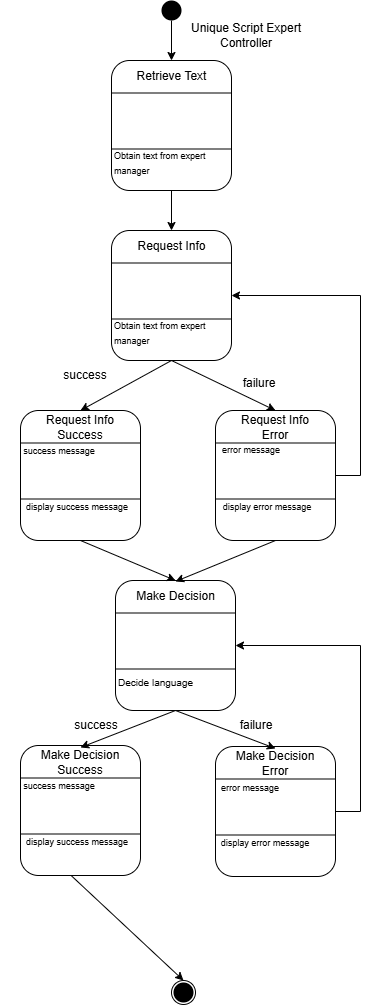
\includegraphics[width=\textwidth, height=0.95\textheight, keepaspectratio]{Section2/images/unique_script_expert_state_diagram.png}
	\caption{Unique Script Expert}
	\label{UniqueScriptExpert}
\end{figure}
\begin{figure}[H]
	\centering
	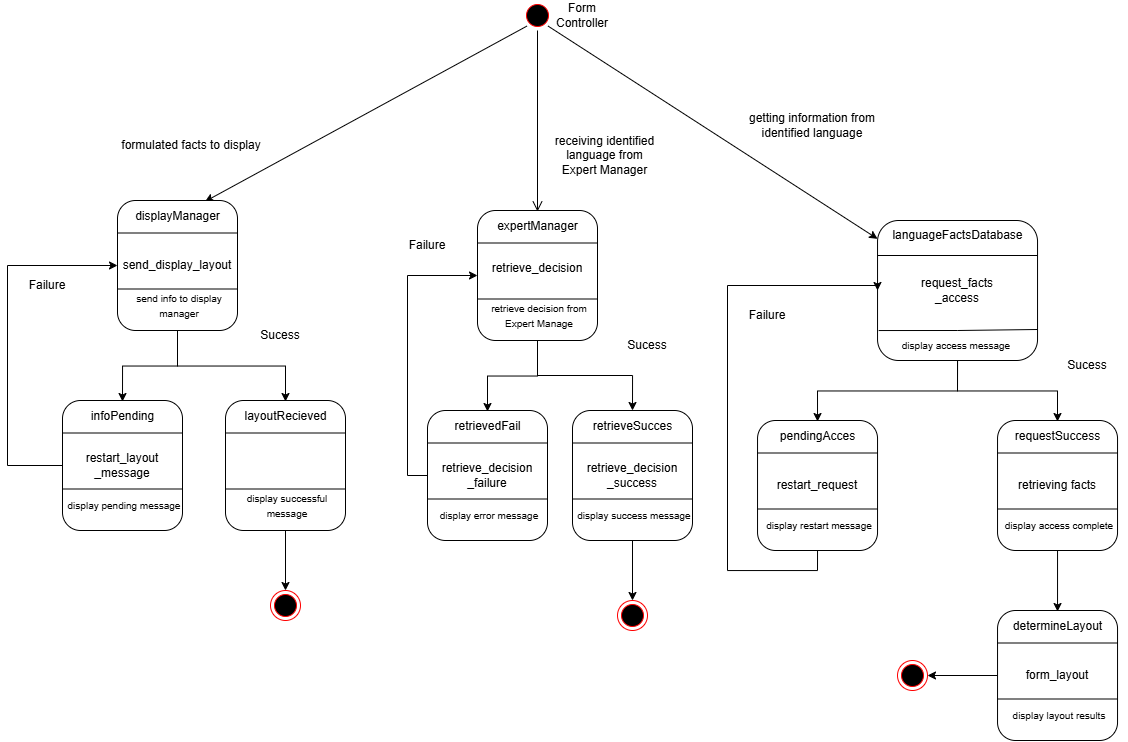
\includegraphics[width=\textwidth, height=\textheight, keepaspectratio]{Section2/images/FormController.png}
	\caption{Form Controller}
	\label{FormController}
\end{figure}

\begin{figure}[H]
	\centering
	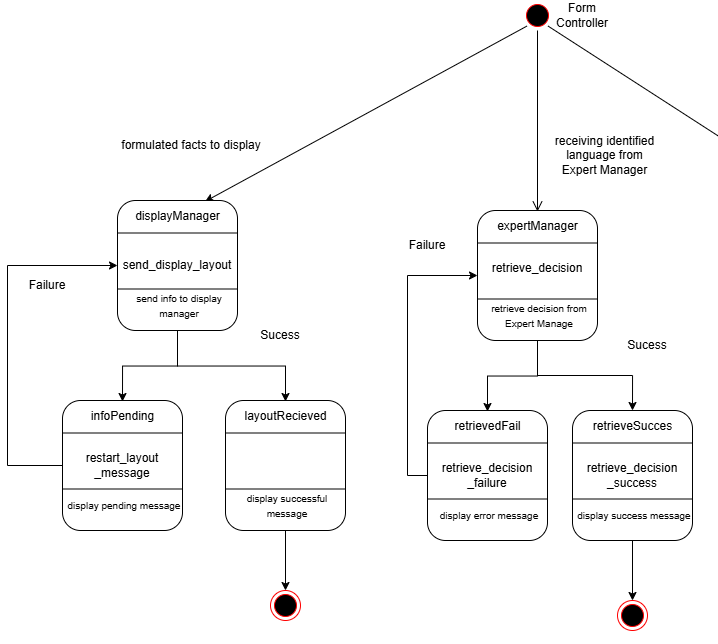
\includegraphics[width=\textwidth, height=\textheight, keepaspectratio]{Section2/images/FormControllerLeftHalf.png}
	\caption{Form Controller Left Half}
	\label{FormController}
\end{figure}

\begin{figure}[H]
	\centering
	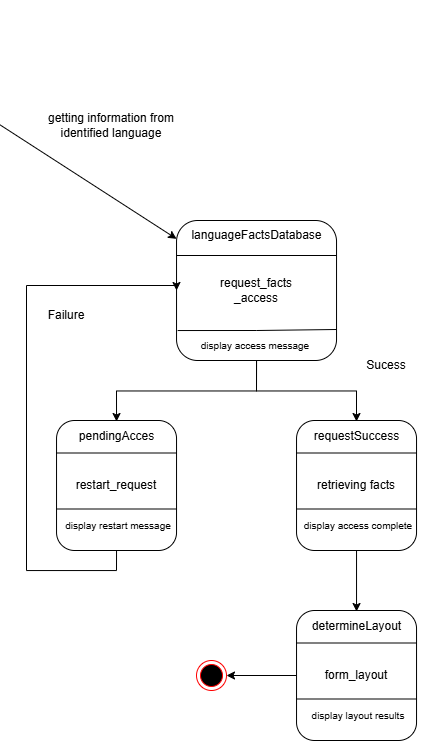
\includegraphics[width=\textwidth, height=\textheight, keepaspectratio]{Section2/images/FormControllerRightHalf.png}
	\caption{Form Controller Right Half}
	\label{FormController}
\end{figure}
\begin{figure}[H]
	\centering
	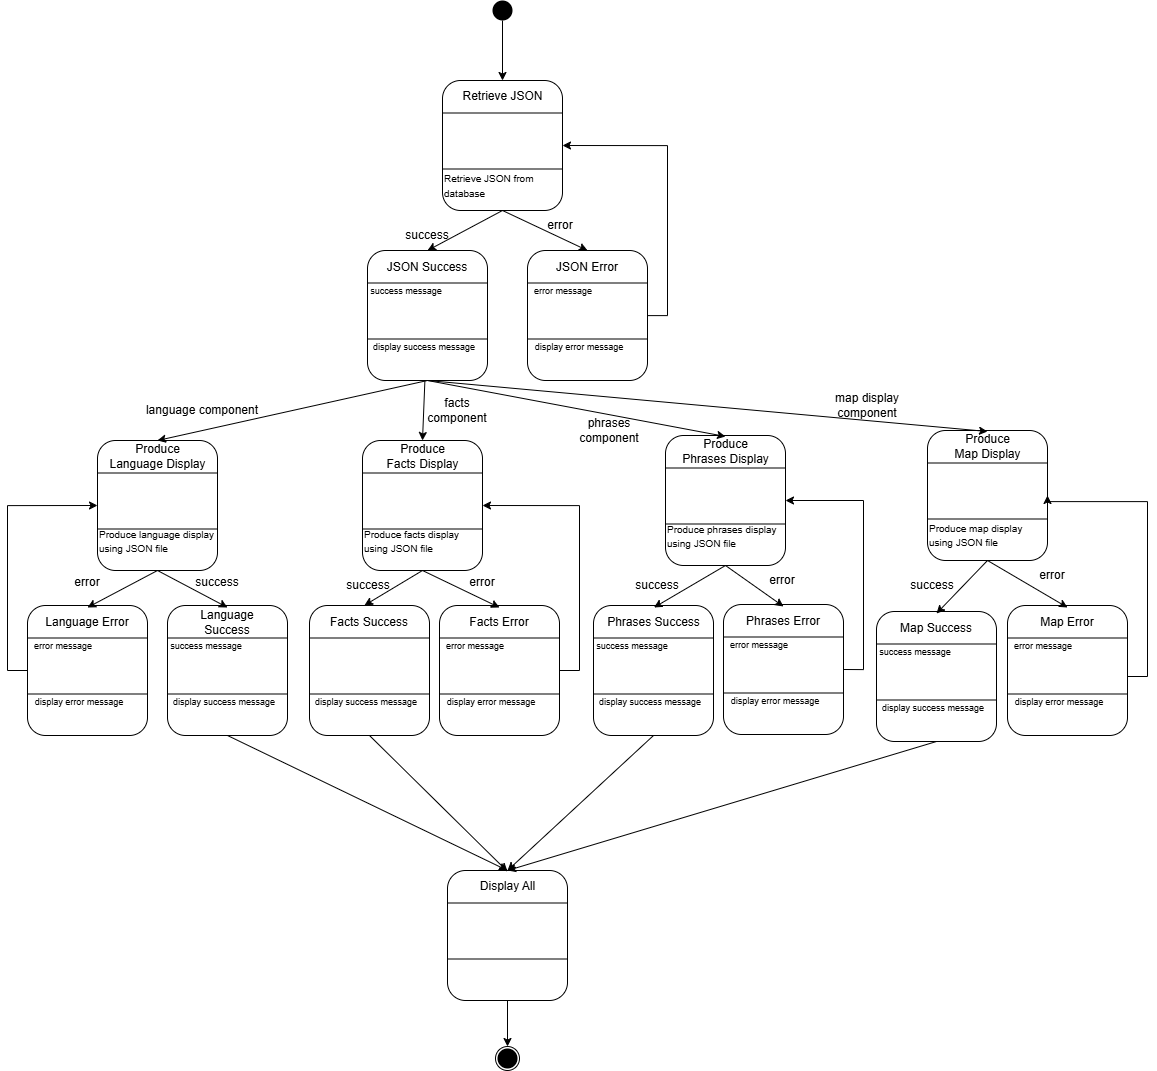
\includegraphics[width=\textwidth, height=\textheight, keepaspectratio]{Section2/images/display_manager_state_diagram.png}
	\caption{Display Manager}
	\label{DisplayManager}
\end{figure}

\begin{figure}[H]
	\centering
	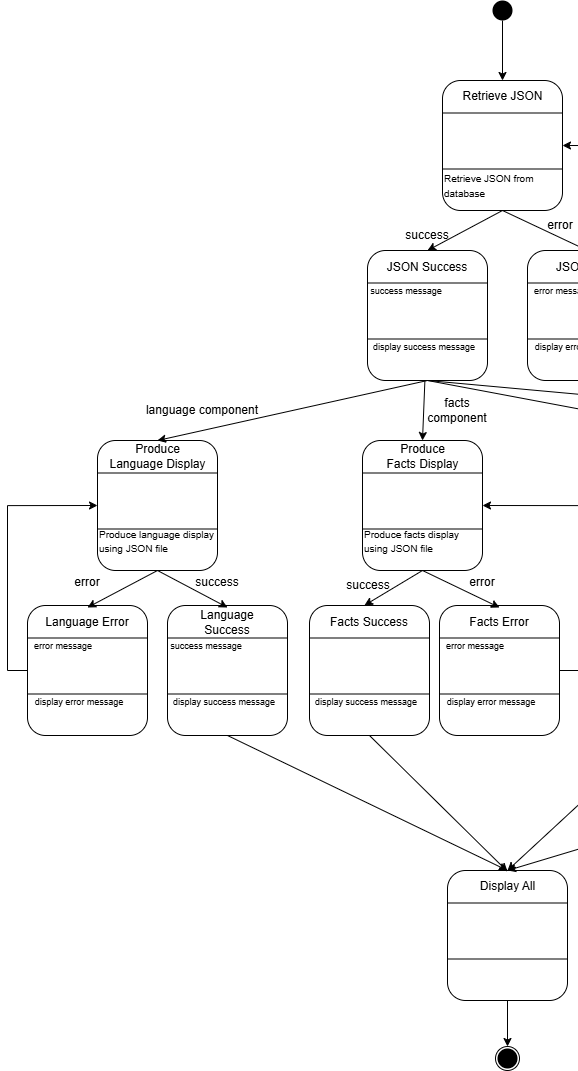
\includegraphics[width=\textwidth, height=\textheight, keepaspectratio]{Section2/images/display_manager_state_diagram_left_half.png}
	\caption{Display Manager Right Half}
	\label{DisplayManager}
\end{figure}

\begin{figure}[H]
	\centering
	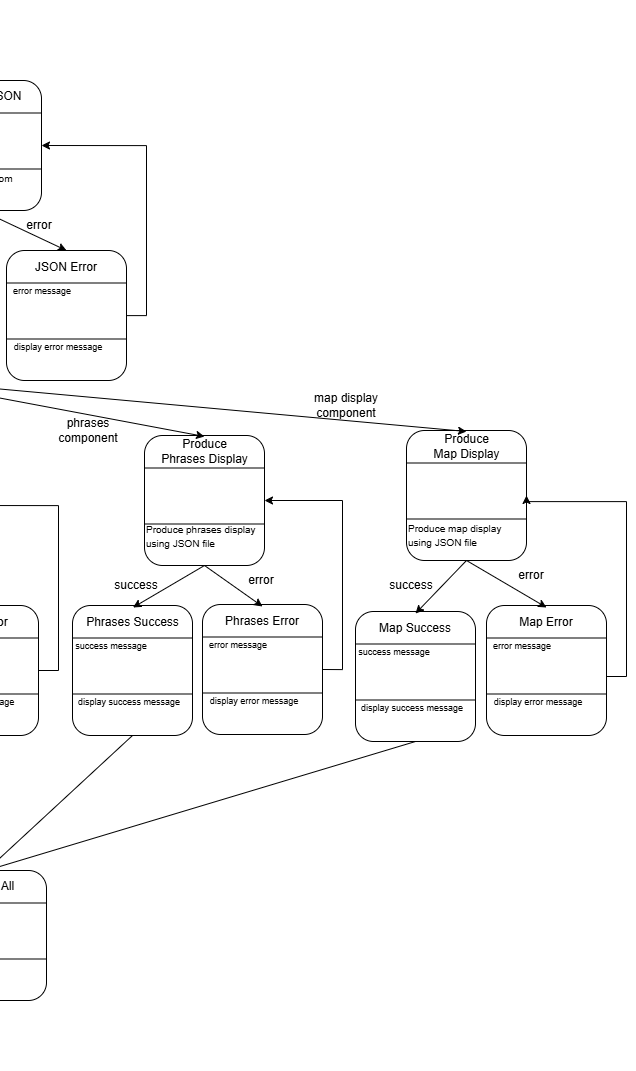
\includegraphics[width=\textwidth, height=\textheight, keepaspectratio]{Section2/images/display_manager_state_diagram_right_half.png}
	\caption{Display Manager Right Half}
	\label{DisplayManager}
\end{figure}
\begin{figure}[H]
	\centering
	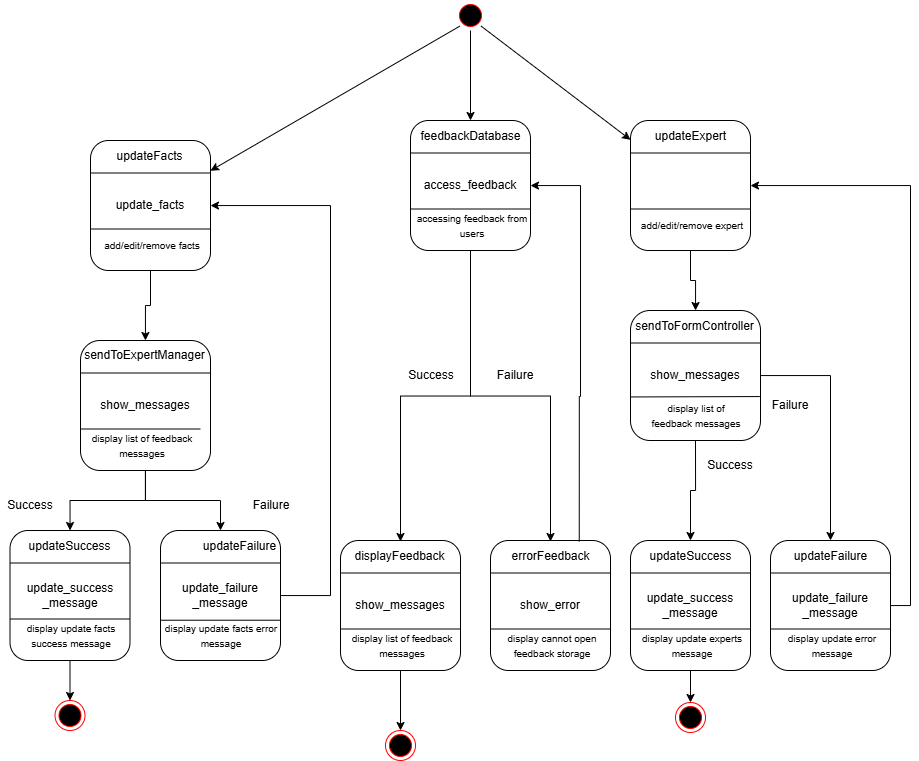
\includegraphics[width=\textwidth, height=\textheight, keepaspectratio]{Section2/images/Admin Console.png}
	\caption{Admin Console}
	\label{AdminConsole}
\end{figure}
\begin{figure}[H]
	\centering
	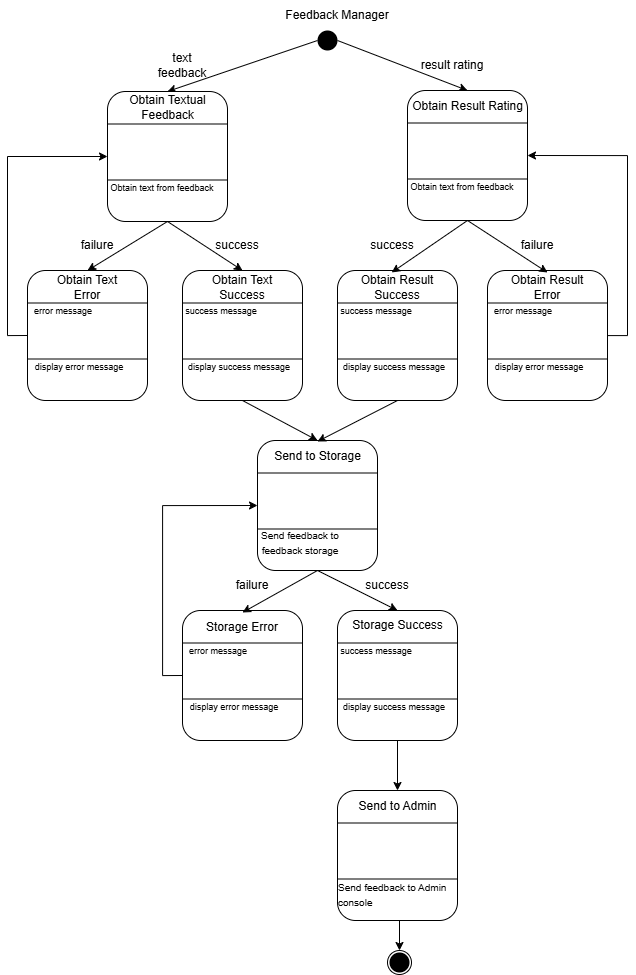
\includegraphics[width=\textwidth, height=0.95\textheight, keepaspectratio]{Section2/images/feedback_manager_state_diagram.png}
	\caption{Feedback Manager}
	\label{FeedbackManager}
\end{figure}



% SECTION 3
\section{Sequence Diagrams}
\label{sec:sequenceDiagrams}

\begin{figure}[H]
	\centering
	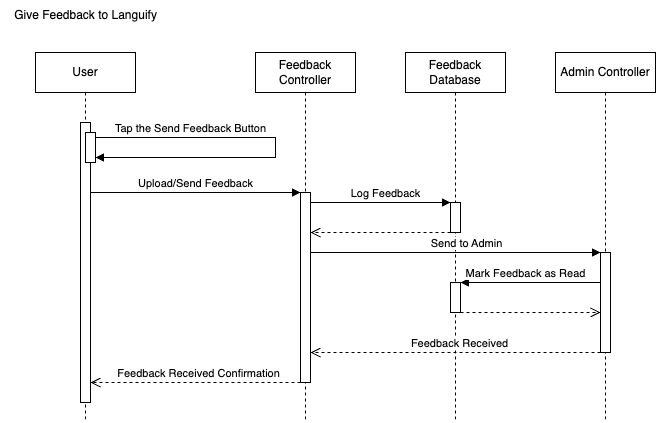
\includegraphics[width=\textwidth, height=\textheight, keepaspectratio]{Section3/images/GiveFeedbackLanguifySequenceDiagram.drawio.png}
	\caption{Feedback Sequence}
	\label{FeedbackSequence}
\end{figure}
\begin{figure}[H]
	\centering
	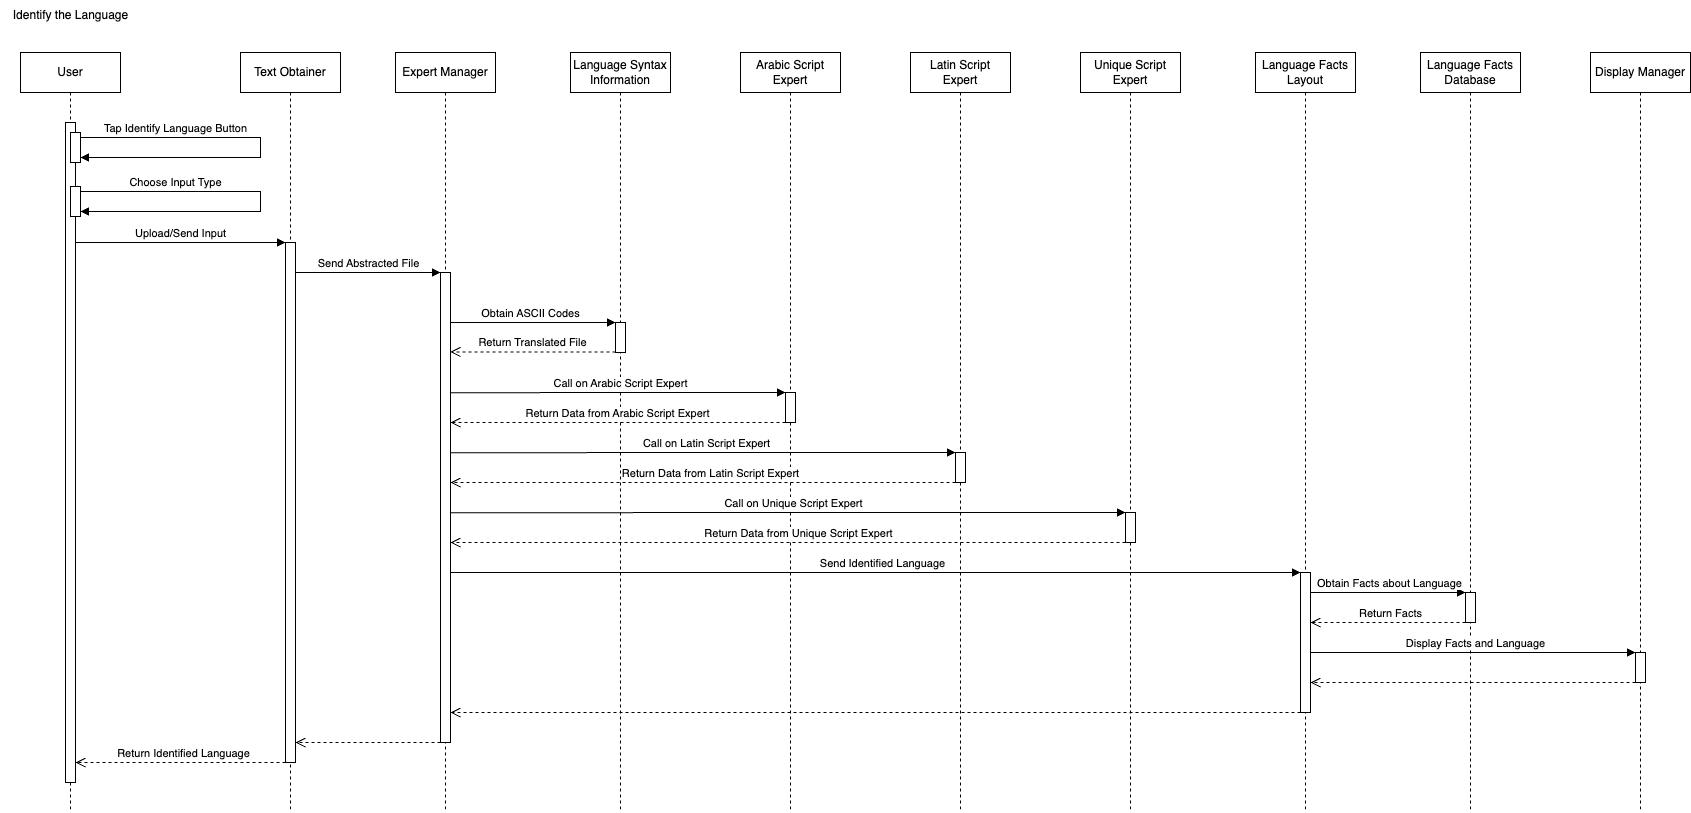
\includegraphics[width=\textwidth, height=\textheight, keepaspectratio]{Section3/images/IdentifyLanguageSequenceDiagram.drawio.png}
	\caption{identify Sequence}
	\label{IdentifySequence}
\end{figure}
\begin{figure}[H]
	\centering
	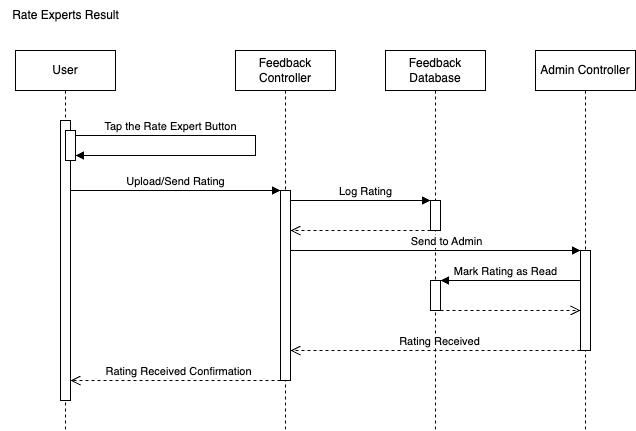
\includegraphics[width=\textwidth, height=\textheight, keepaspectratio]{Section3/images/RateExpertsResultSequenceDiagram.drawio.png}
	\caption{Rate Expert Sequence}
	\label{RateExpertSequence}
\end{figure}
\begin{figure}[H]
	\centering
	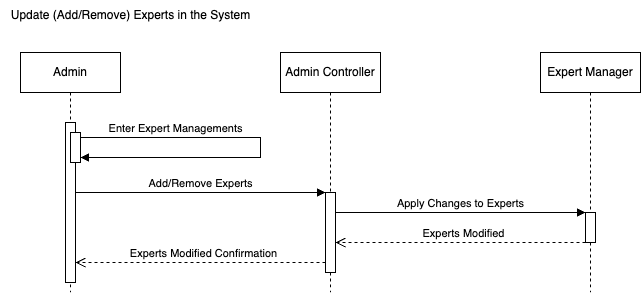
\includegraphics[width=\textwidth, height=\textheight, keepaspectratio]{Section3/images/UpdateExpertsSequenceDiagram.drawio.png}
	\caption{Update Expert Sequence}
	\label{UpdateExpertSequence}
\end{figure}
\begin{figure}[H]
	\centering
	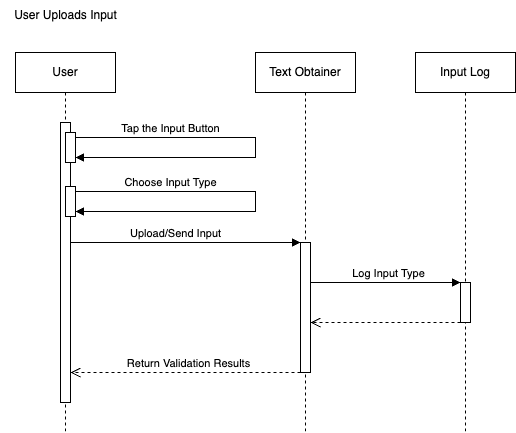
\includegraphics[width=\textwidth, height=\textheight, keepaspectratio]{Section3/images/UserUploadsInputSequenceDiagram.drawio.png}
	\caption{User Upload Input Sequence}
	\label{UserUploadsInputSequence}
\end{figure}


% SECTION 4
\section{Detailed Class Diagram}
\label{sec:detailed_class_diagram}

\begin{figure}[H]
	\centering
	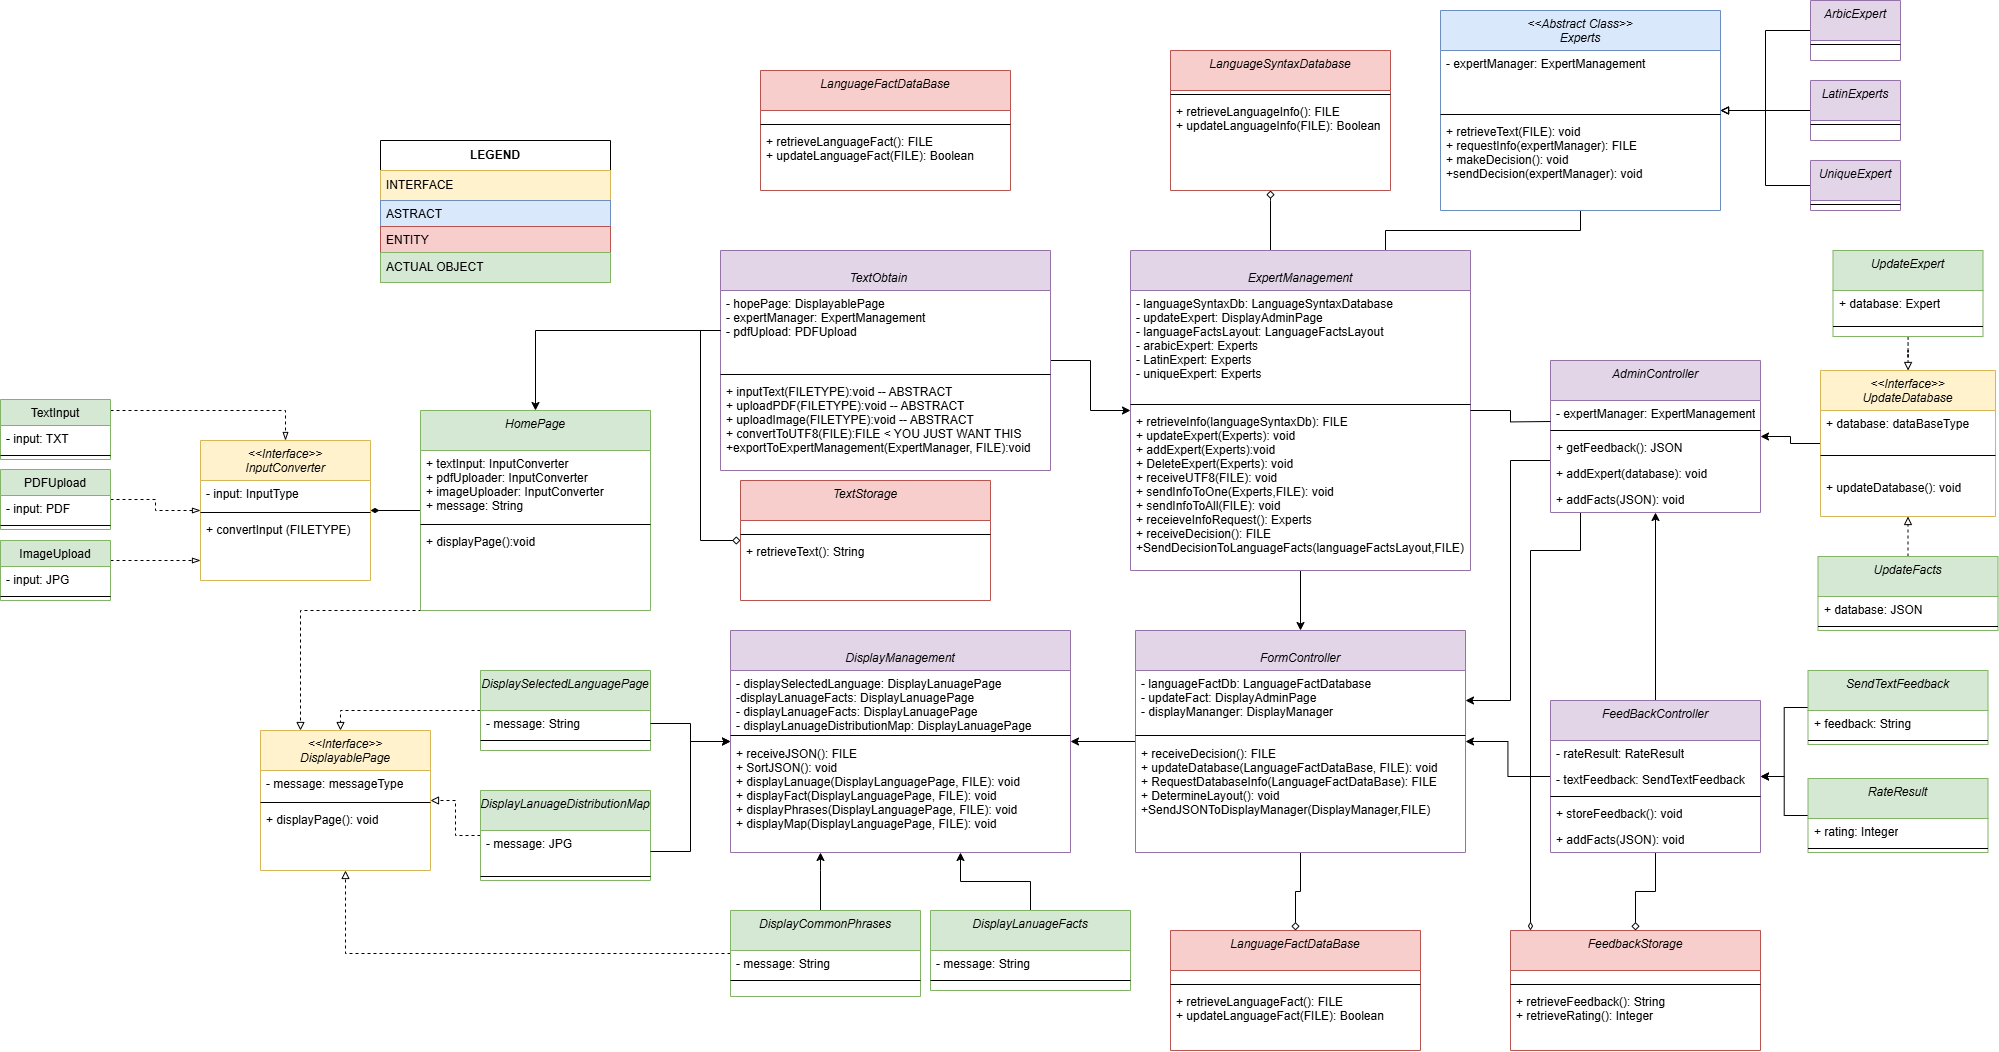
\includegraphics[width=\textwidth, height=\textheight, keepaspectratio]{Section4/images/LangufiyClassDiagramV5.png}
	\caption{Detailed Class Diagram}
	\label{DetailedClassDiagram}
\end{figure}

\begin{figure}[H]
	\centering
	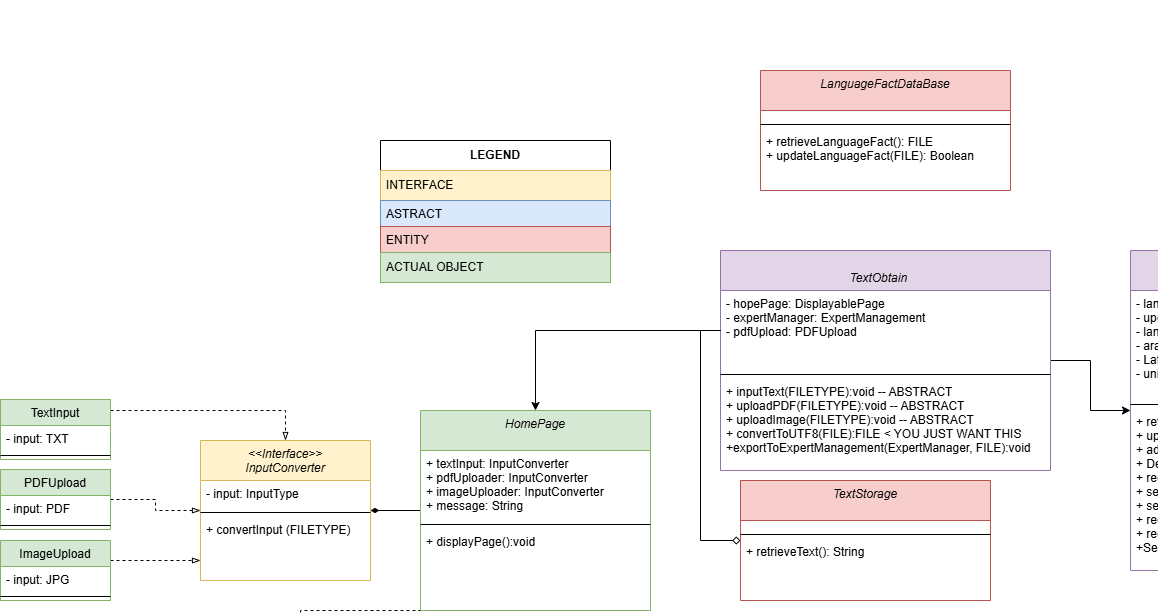
\includegraphics[width=\textwidth, height=\textheight, keepaspectratio]{Section4/images/LangufiyClassDiagramV5Q1.png}
	\caption{Detailed Class Diagram Quandrant 1}
	\label{DetailedClassDiagramQ1}
\end{figure}

\begin{figure}[H]
	\centering
	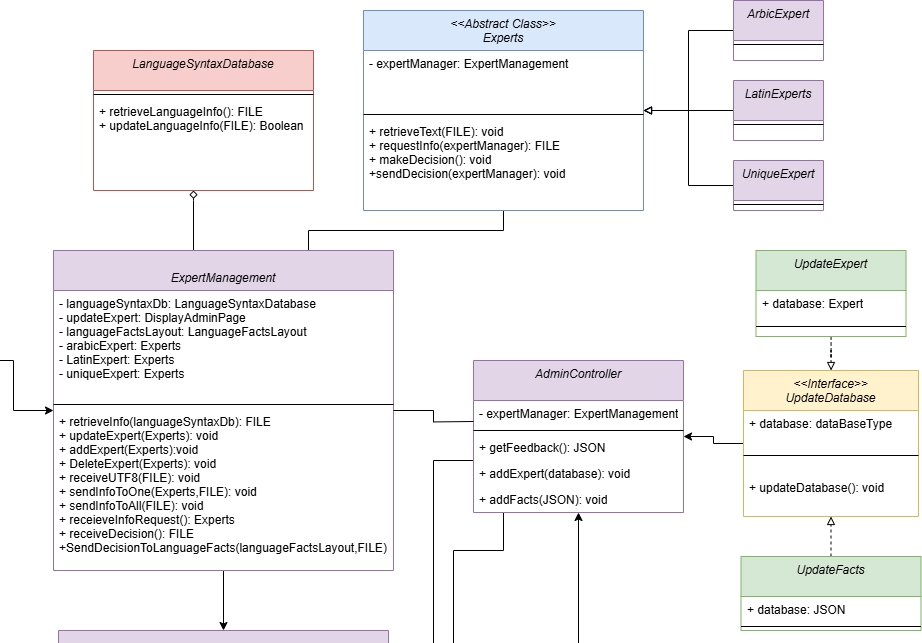
\includegraphics[width=\textwidth, height=\textheight, keepaspectratio]{Section4/images/LangufiyClassDiagramV5Q2.png}
	\caption{Detailed Class Diagram Quandrant 2}
	\label{DetailedClassDiagramQ2}
\end{figure}

\begin{figure}[H]
	\centering
	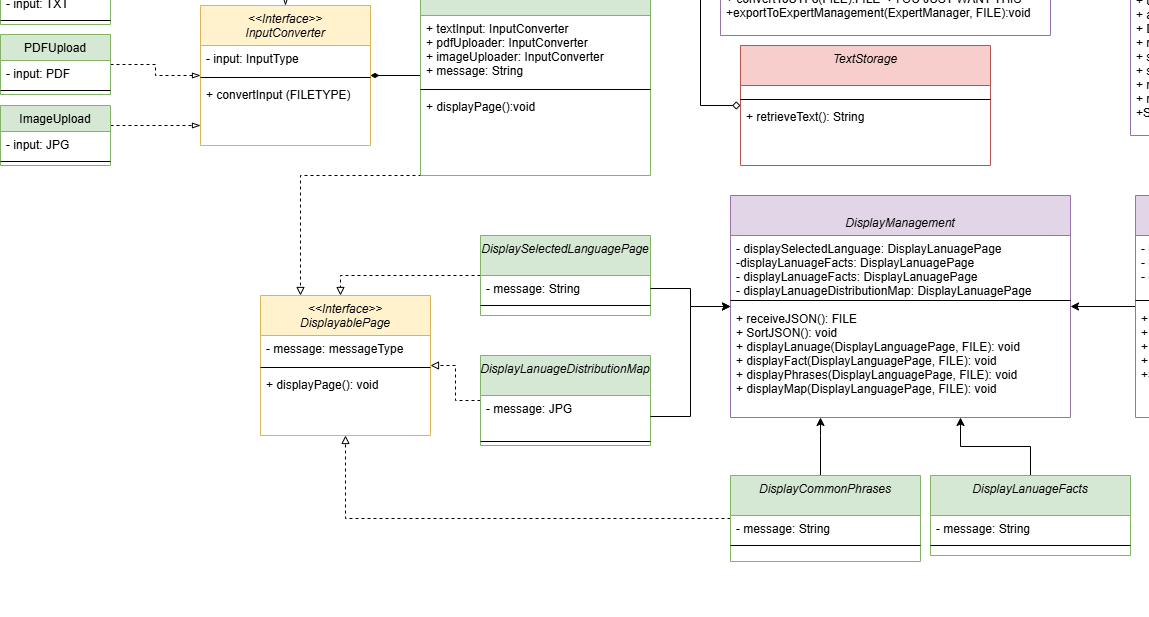
\includegraphics[width=\textwidth, height=\textheight, keepaspectratio]{Section4/images/LangufiyClassDiagramV5Q3.png}
	\caption{Detailed Class Diagram Quandrant 3}
	\label{DetailedClassDiagramQ3}
\end{figure}

\begin{figure}[H]
	\centering
	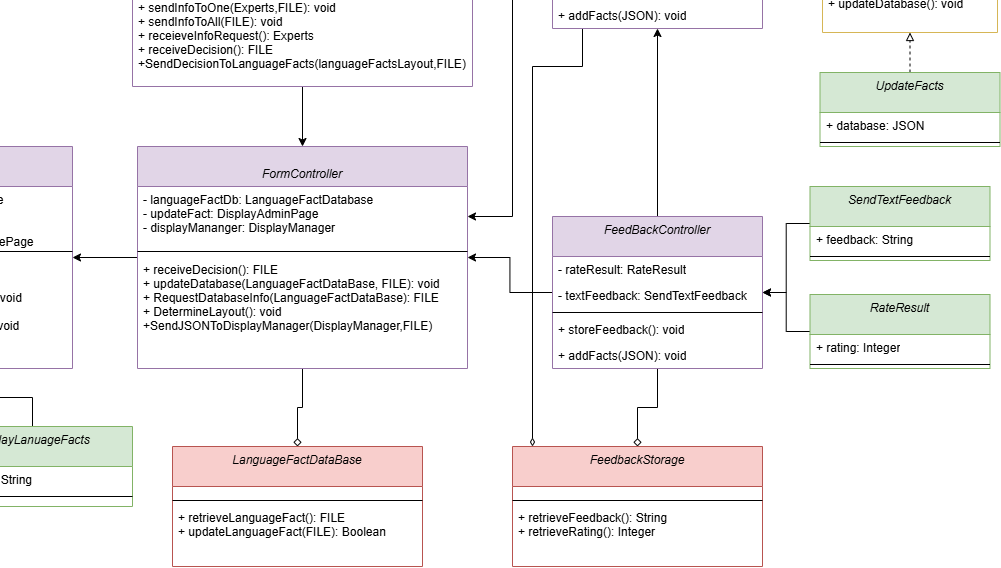
\includegraphics[width=\textwidth, height=\textheight, keepaspectratio]{Section4/images/LangufiyClassDiagramV5Q4.png}
	\caption{Detailed Class Diagram Quandrant 4}
	\label{DetailedClassDiagramQ4}
\end{figure}


% SECTION 5


% SECTION 6


% DIVISION OF LABOR
\appendix
\section{Division of Labour}
\label{sec:division_of_labour}
% Begin Section

\textbf{Andy Huynh}
\begin{itemize}
    \item Worked on Section 4 Business Events with Ke Ma
    \item Set up and translated all the text into the LaTeX file
    \item Worked on Sections 5.5, 5.6, and 5.7 with Ke Ma
\end{itemize}
\begin{figure}[H]
	\centering
	
\includegraphics[width=0.2\textwidth]{Signatures/a.png}  
\end{figure}

\textbf{Cheukman Zhou}
\begin{itemize}
    \item Worked on Section 1.2
    \item Worked on Section 3.1
    \item Helped with formatting and editing of the document on LaTeX
\end{itemize}
\begin{figure}[H]
	\centering
	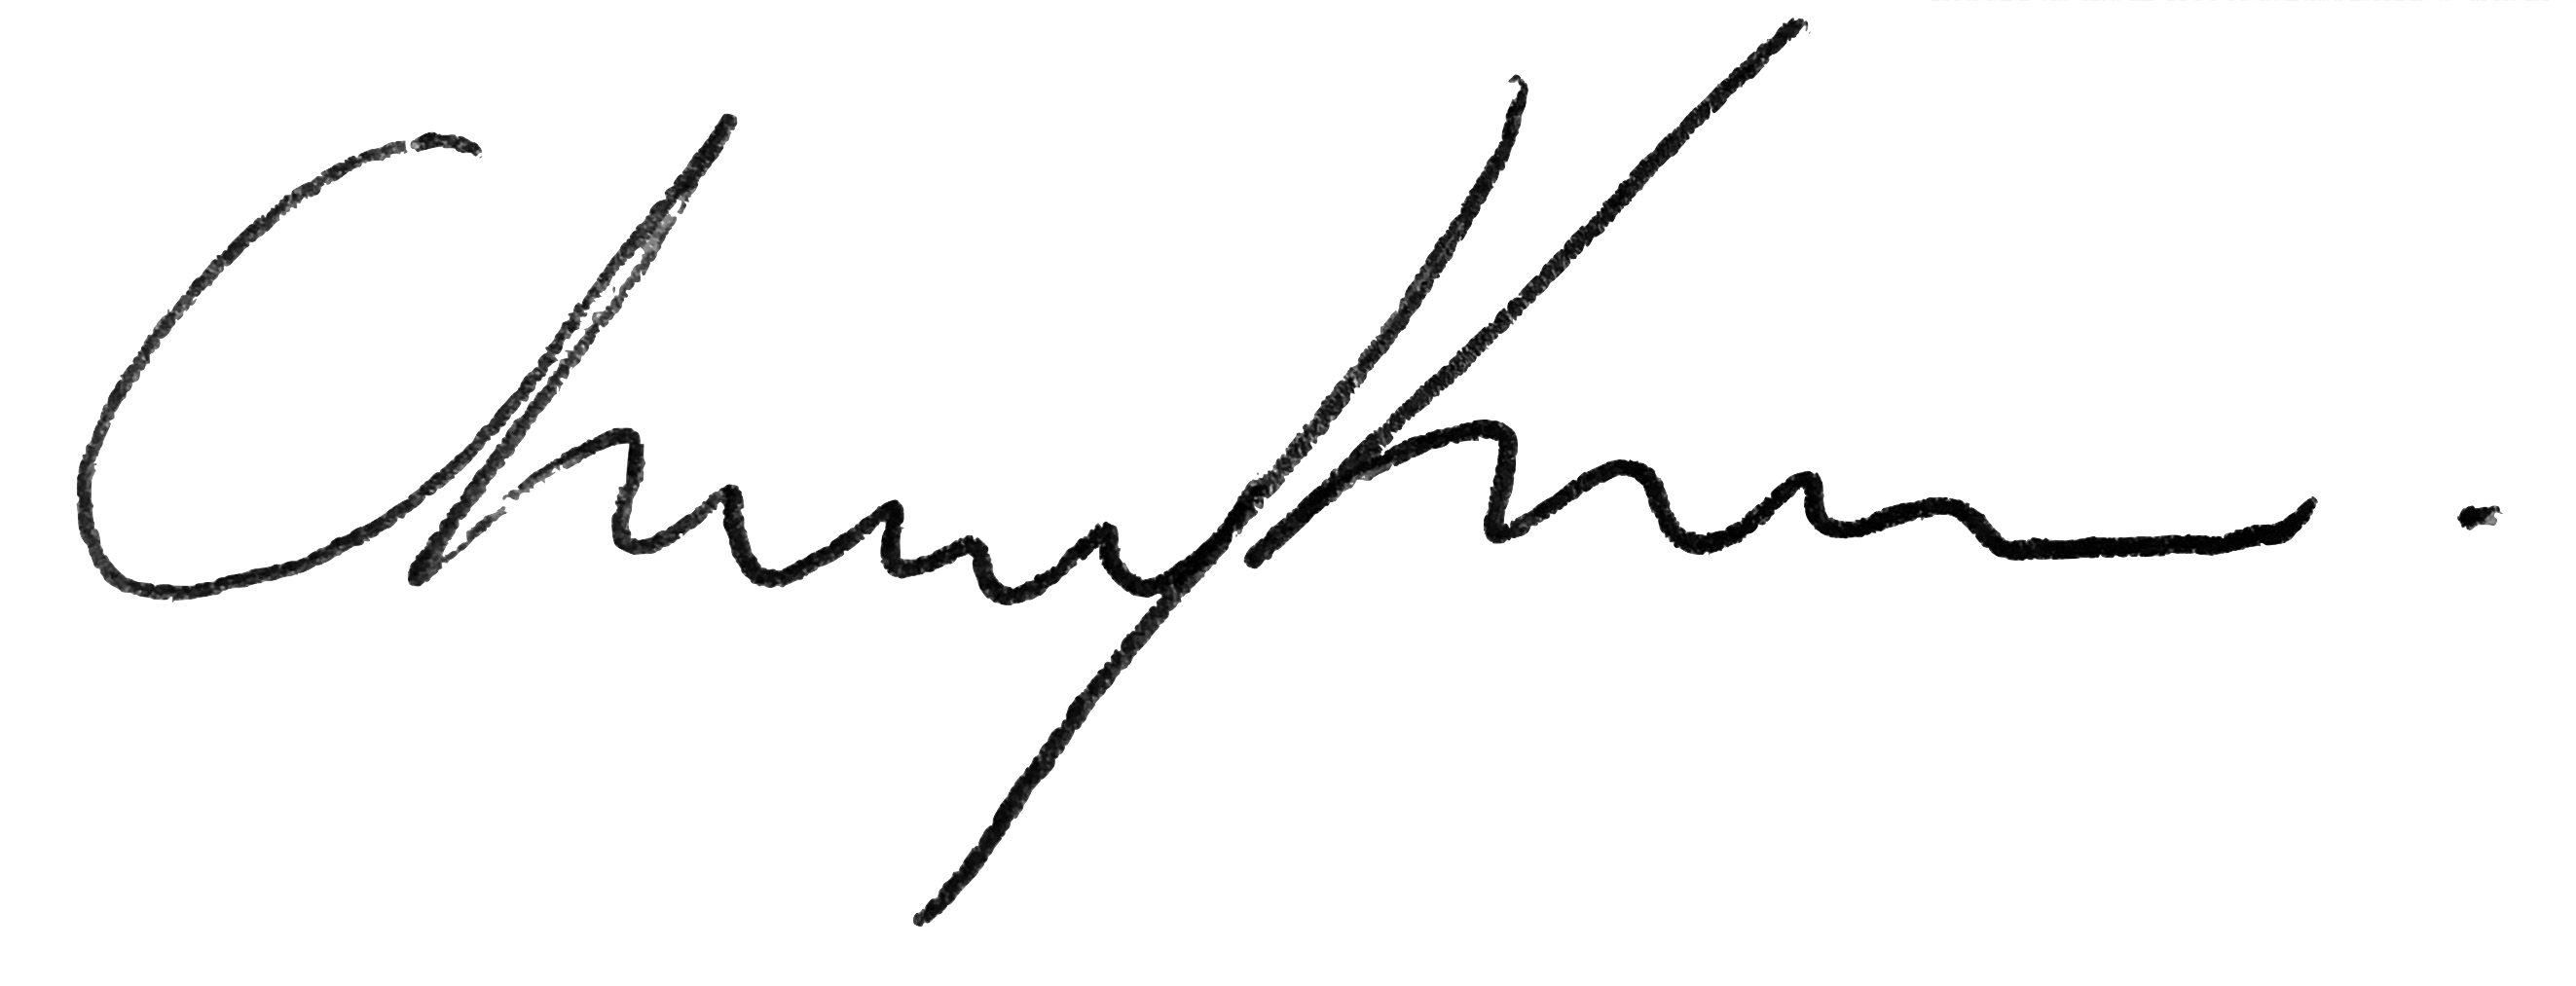
\includegraphics[width=0.2\textwidth]{Signatures/c.png}
\end{figure}

\textbf{Ke Ma}
\begin{itemize}
    \item Worked on Section 4 with Andy Huynh
    \item Worked on Sections 5.5, 5.6, and 5.7 with Andy Huynh
\end{itemize}
\begin{figure}[H]
	\centering
	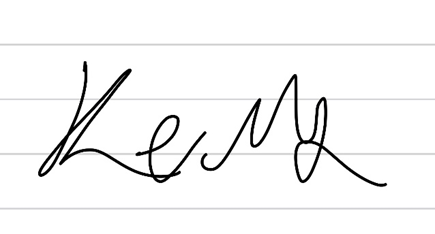
\includegraphics[width=0.2\textwidth]{Signatures/k.png}
\end{figure}

\textbf{Sarah Dorfman}
\begin{itemize}
    \item Worked on Section 2 alongside Cheukman Zhou
    \item Worked on Section 5.1
\end{itemize}
\begin{figure}[H]
	\centering
	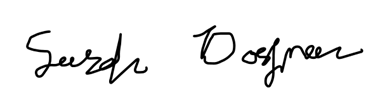
\includegraphics[width=0.2\textwidth]{Signatures/s.png}
\end{figure}

\textbf{Gurmanjot Minhas}
\begin{itemize}
    \item Worked on Section 3
    \item Worked on Sections 5.4 and 5.8
    \item Completed Section 6: Innovative Ideas
\end{itemize}
\begin{figure}[H]
	\centering
	
\includegraphics[width=0.2\textwidth]{Signatures/g.png}
\end{figure}

% End Section


\end{document}
%------------------------------------------------------------------------------